\let\negmedspace\undefined
\let\negthickspace\undefined
\documentclass[journal]{IEEEtran}
\usepackage[a5paper, margin=10mm, onecolumn]{geometry}
\usepackage{lmodern} % Ensure lmodern is loaded for pdflatex
\usepackage{tfrupee} % Include tfrupee package

\setlength{\headheight}{1cm} % Set the height of the header box
\setlength{\headsep}{0mm}     % Set the distance between the header box and the top of the text

\usepackage{gvv-book}
\usepackage{gvv}
\usepackage{cite}
\usepackage{amsmath,amssymb,amsfonts,amsthm}
\usepackage{algorithmic}
\usepackage{graphicx}
\usepackage{textcomp}
\usepackage{xcolor}
\usepackage{txfonts}
\usepackage{listings}
\usepackage{enumitem}
\usepackage{mathtools}
\usepackage{gensymb}
\usepackage{comment}
\usepackage[breaklinks=true]{hyperref}
\usepackage{tkz-euclide} 
\usepackage{listings}
\def\inputGnumericTable{}                                 
\usepackage[latin1]{inputenc}                                
\usepackage{color}                                            
\usepackage{array}                                            
\usepackage{longtable}                                       
\usepackage{calc}                                             
\usepackage{multirow}                                         
\usepackage{hhline}                                           
\usepackage{ifthen}                                           
\usepackage{lscape}

\begin{document}

\bibliographystyle{IEEEtran}
\vspace{3cm}

\title{12.8.1.12}
\author{EE24BTECH11030 - KEDARANANDA}
% \maketitle
% \newpage
% \bigskip
{\let\newpage\relax\maketitle}

\renewcommand{\thefigure}{\theenumi}
\renewcommand{\thetable}{\theenumi}
\setlength{\intextsep}{10pt} % Space between text and floats

\textbf{Question:}
 Area lying in the first quadrant and bounded by the circle $x^{2} + y^{2} = 4$ and the lines.x = 0 and x = 2 is\\

\textbf{Solution:}\\\\
\textbf{Theoritical Solution:}
\begin{align}
 A &= \int_0^2 \sqrt{4 - x^2} \, dx. 
\end{align}
Substitute x = 2$\sin \theta$\\
\begin{align}
A &= \int_0^{\pi/2} 2 \cos \theta \cdot 2 \cos \theta \, d\theta \\
&= \int_0^{\pi/2} 4 \cos^2 \theta \, d\theta. 
\end{align}
Using the identity  $\cos^2 \theta = \frac{1 + \cos 2\theta}{2}$\\
\begin{align}
A &= \int_0^{\pi/2} 4 \cdot \frac{1 + \cos 2\theta}{2} \, d\theta \\
&= \int_0^{\pi/2} 2 \, d\theta + \int_0^{\pi/2} 2 \cos 2\theta \, d\theta. 
\end{align}
\begin{align}
\int_0^{\pi/2} 2 \, d\theta &= 2 \left[ \theta \right]_0^{\pi/2} = 2 \cdot \frac{\pi}{2} - 0 = \pi, \\
\int_0^{\pi/2} 2 \cos 2\theta \, d\theta &= \left[ \sin 2\theta \right]_0^{\pi/2} = \sin \pi - \sin 0 = 0. \\
\end{align}
Thus, the area is: $A = \pi + 0 = \pi$.\\\\
\textbf{Computational Solution:}\\
We need to compute  A = $\int_0^2 \sqrt{4 - x^2} \, dx$ using the trapezoidal rule with n = 500.The interval is  [a, b] = [0, 2]  and the number of subintervals is  n = 500.

\begin{align}
\text{The width of each subinterval is } h = \frac{b - a}{n} = \frac{2 - 0}{500} = 0.004.
\end{align}
\begin{align}
\text{The function to integrate is f(x)} = \sqrt{4 - x^2}.
\end{align}

\begin{align}
\text{The trapezoidal rule formula is: } A \approx h \left[ \frac{1}{2} f(a) + f(x_1) + f(x_2) + \dots + f(x_{n-1}) + \frac{1}{2} f(b) \right].
\end{align}
The points  $x_i$  are given by
\begin{align}
  x_i = a + i h = 0 + i \cdot 0.004, \text{ for } i = 0, 1, 2, \dots, 500.
\end{align}
\begin{align}
\text{Substitute the values: } A \approx 0.004 \left[ \frac{1}{2} f(0) + f(x_1) + f(x_2) + \dots + f(x_{499}) + \frac{1}{2} f(2) \right].
\end{align}

\begin{align}
\text{Compute } f(0) = \sqrt{4 - 0^2} = 2, \text{ and } f(2) = \sqrt{4 - 2^2} = 0.
\end{align}

\begin{align}
\text{Summing the terms and applying the formula, we find } A \approx 3.1415.
\end{align}
\begin{figure}[h!]
   \centering
   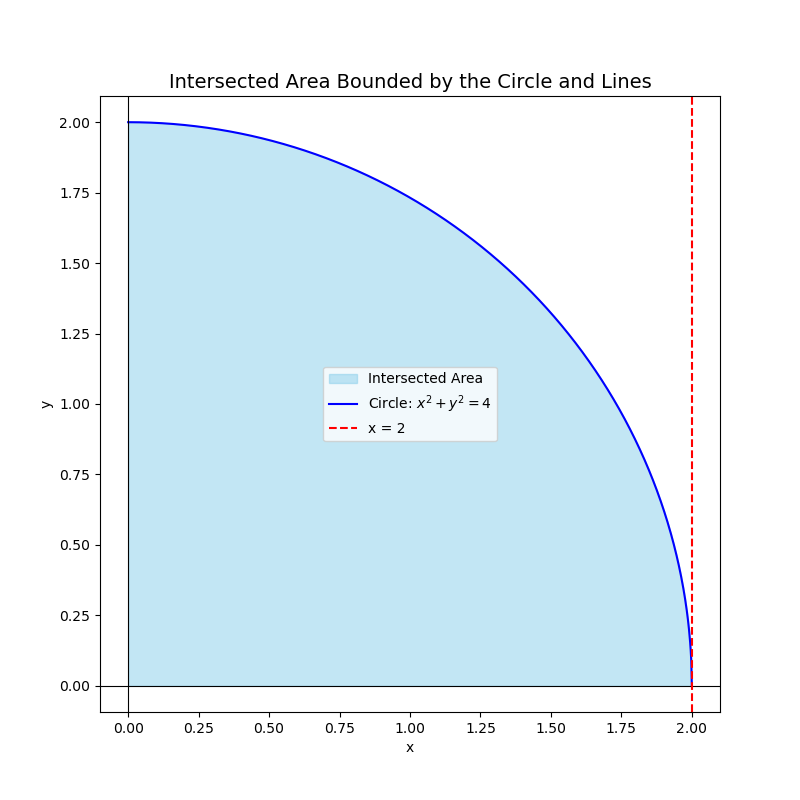
\includegraphics[width=\columnwidth]{figs/Fig1.png}
\end{figure}
\end{document}

